\documentclass[letterpaper, 11pt]{article}
\usepackage{amsmath}
\usepackage{amssymb}
\usepackage{float}
\usepackage{inputenc}
\usepackage[left=2cm, right=2cm, top=2cm, bottom=2cm]{geometry}
\usepackage{graphicx}
\usepackage{float}
\usepackage{caption}
\usepackage{extarrows}
\usepackage{xcolor}
\usepackage{lscape}
\usepackage{pdflscape}
\usepackage{pdfpages}
\usepackage{multicol}
\usepackage{leftindex}
\usepackage{algorithm2e}
\SetKwComment{Comment}{/* }{ */}
%\RestyleAlgo{ruled}
\usepackage{mathtools}
\usepackage{hyperref}
\hypersetup{
    colorlinks=false,
    }

% Listings
\usepackage{listings}
\usepackage{color}
\input{lst_style.tex}

% NewCommands
\newcommand{\peq}{ \mathrel{+}= }
\newcommand{\muleq}{ \mathrel{*}= }
\newcommand{\sign}{\,\text{sign}}
\newcommand{\bm}[1]{\begin{bmatrix} #1 \end{bmatrix}}
\newcommand{\lx}[2]{\leftindex #1 {#2}}
\newcommand{\norm}[1]{\left\lvert #1 \right\rvert}
\newcommand{\abs}[1]{\norm{#1}}
\newcommand{\itbf}[1]{\textit{\textbf{#1}}}
\newcommand{\mdet}[1]{\norm{\begin{matrix} #1 \end{matrix}}}
\newcommand{\lr}[1]{\left( #1 \right)}
\newcommand{\sat}{\,\text{sat}}



\title{Identification and Control of Multirotor Actuator Dynamics with RPM feedback}
\author{Sesha Charla}
\date{\today}


\begin{document}
\maketitle
\tableofcontents
%===============================================================================
\newpage
\part{Model Parameter Identification}
\section{Brushless DC motor model}
\input{./secs/1_1-bldc_static.tex}
\subsection{Dynamic Model (without Propeller)}
We have the dynamic model of BLDC motor using moment balance:
\begin{align*}
    J_m \dot \omega_m &= T_e - b_f \omega_m - M_f\\
    \text{where, } \qquad &\\
    J_m &- \text{Moment of inertia of the motor}\\
    b_f &- \text{lumped parameter for viscous friction}\\
    M_f &- \text{lumped parameter for coulomb friction}
\end{align*}
\itbf{Friction:}
\begin{enumerate}
    \item Viscous friction: $-b_f \omega$.
    \item Columb friction: $-M_{f} \sign(\omega) = -M_{f} \qquad [\because$ the motor turns in only one direction $]$.
\end{enumerate}

\medskip

From the speed-torque characteristics of the BLDC motor:
\begin{align*}
    T_e &= K_T I = K_T \frac{(V_s - E)}{R} = \frac{K_T}{R} (V_s - K_v \omega_m)  & [\because K_v = K_T = k \psi]\\
    \text{Let, }\qquad \qquad &\\
    K_r &= \frac{K_T}{R}
\end{align*}
From the definition of Input to ESC:
\begin{align*}
    V_s &= u V_{in}\\
    \therefore T_e &= u K_r V_{in} - K_r K_v \omega_m
\end{align*}

Substituting:
\begin{align*}
    &J_m \dot \omega_m = u K_r V_{in}  - K_rK_v \omega_m  - b_f \omega_m - M_f
    & Let \\
    & b_{m} = K_r K_v  + b_f
\end{align*}
\begin{equation}
    \boxed{
    J_m \dot \omega_m + b_m \omega_m + M_f = u K_r V_{in}
    }
    \label{eqn:no_prop}
\end{equation}

\subsection{BLDC Motor with Propeller}
Adding propeller moment of inertia and the moment due to propeller drag into the BLDC motor model.
\begin{align*}
    (J_m + J_p) \dot \omega + b_m \omega + M_f &= u K_r V_{in} - C_D \omega^2
\end{align*}
Where, $C_D$ is the aerodynamic drag. Let, $J_m + J_p = J$
\begin{equation}
    \boxed{
    J\dot \omega + b_m \omega + C_D \omega^2 + M_f = u K_r V_{in}
    }
    \label{eqn:prop}
\end{equation}

\subsection{Propeller Aerodynamics}
Aerodynamics are assumed to be faster than mechanical dynamics of the actuator.
The thrust generation process due to the propagation of pressure wave is assumed to be instantaneous. This assumption is inherent to the standard models that use potential flow theory (lifting-line, blade-element and momentum-disk theories), as they assume incompressible flow.\\

\begin{minipage}{0.49\textwidth}
    \itbf{Propeller Thrust}:
    \begin{align*}
        F_T = C_{T} \omega^2
    \end{align*}

    \itbf{Propeller moment due to drag}:
    \begin{align*}
        M_D = C_{D} \omega^2
    \end{align*}
\end{minipage}
\begin{minipage}{0.49\textwidth}
    \begin{figure}[H]
        \centering
        \includegraphics[width = \textwidth]{figs/aero/expt_setup.eps}
        \caption{Experimental Setup}
        \label{fig:expt_setup}
    \end{figure}
\end{minipage}

\bigskip

\textbf{Aeroelasticity of the propeller:} It is assumed that the aeroelasticity of the propeller produces high-frequency oscillations in the thrust and torque of the propller which are assumed to be very fast and roll off w.r.t the mechanical dyanmics dyanmics of the actuator as well as the transmission through the propller shaft. The constant  bias in the torque due to flutter is captured in the drag coefficient and it's parameter uncertainity.\\


\subsubsection{Parameter estimation form the static data}

In the experimental setup (Figure~\ref{fig:expt_setup}),  the total moment measured is the result of aerodynamic moment and the friction of the BLDC motor. Thus the total moment becomes:
\begin{align*}
    M = C_D \omega^2 + b_f \omega + M_f
\end{align*}

The aerodynamic coefficients are estimated from the static measuremnts using least-squares estimation.

\begin{figure}[H]
    \begin{minipage}{0.49\textwidth}
        \begin{figure}[H]
            \centering
            \includegraphics[width = \textwidth]{./figs/aero/Thrust_curve.eps}
        \end{figure}
        \caption{Variation of thrust with rpm}
    \end{minipage}
    \begin{minipage}{0.49\textwidth}
        \begin{figure}[H]
            \centering
            \includegraphics[width = \textwidth]{./figs/aero/Drag_curve.eps}
            \caption{Variation of drag moment with rpm}
        \end{figure}
    \end{minipage}
\end{figure}

The moment data has more variation from model due to the unmodelled aerodynamic effects such as aerodynamic-flutter. Thus we have the estimates of force coefficients:

\begin{table}[H]
    \centering
    \begin{tabular}{c l}
        \hline \hline
        Parameter & Value \\ \hline \hline
        $C_T$ & $7.2581 \times 10^{-06}$ $N/(rad/s)^2$  \\
        $C_D$ & $3.6088 \times 10^{-08}$ $N.m/(rad/s)^2$ \\
        $b_f$ & $0.0$ $N.m/(rad/s)$\\
        $M_f$ & $1.3135 \times 10^{-3}$ $N.m$\\ \hline \hline
    \end{tabular}
    \caption{Estimates Force coefficients}
\end{table}

%===============================================================================
\newpage
\section{RPM Measurement}
\input{secs/2-rpm_feedback.tex}
%===============================================================================
\newpage
\section{Input definition and Static Calibration}
\input{./secs/3_1-ESC_input.tex}
\subsection{Normalized Angular Velocity Input}

We have the no-load dynamic model for the BLDC motor with propeller:
\begin{align*}
    J \dot \omega + b_m \omega + C_D \omega^2+ M_f &= u K_r V_{in}
\end{align*}
At steady state ($\dot \omega = 0$), the above equation becomes:
\begin{align*}
    b_m \omega + C_D \omega^2 +  M_f &= u K_r V_{in}\\
    \implies \frac{b_m}{K_r} \left(\frac{\omega_m}{V_{in}}\right) + \frac{V_{in}}{K_r} C_D \lr{\frac{\omega}{V_{in}}}^2 + \frac{M_f}{K_r V_{in}} &= u
\end{align*}

\itbf{Definition}: Let, $u_{\omega}$ be the angular velocity of the motor with propeller at unit supply voltage for the given pwm input ($u_p$). Also, let us call it "\itbf{Normalized angular velocity}".
\begin{align*}
    u_{\omega} &= \frac{\omega}{V_{in}} \text{  at  } u = g_u(u_p)\\
    \implies u &= \underbrace{\frac{b_m}{K_r} u_\omega + \frac{\hat V_{in}}{K_r} C_D u_\omega^2 + \frac{M_f}{K_r  \hat V_{in}}}_{g_\omega (u_\omega, \hat V_{in})}
\end{align*}

The relationship between $u_\omega$ and $u_p$ can be estimated from the staic measuremnt data.
\begin{figure}[H]
    \begin{minipage}{0.49\textwidth}
    We have:
        \begin{align*}
            u_\omega &= a u_p + b
            \qquad a = 0.0696
            \qquad b = -64.3266\\
        \end{align*}
    Also,
        \begin{align*}
            \because u &= g_\omega(u_\omega, \hat V_{in})\\
            \implies g_u(u_p) &= g_\omega(a u_p  + b, \hat V_{in})\\
        \end{align*}
    \end{minipage}
    \begin{minipage}{0.49\textwidth}
       \begin{figure}[H]
            \centering
            \includegraphics[width = \textwidth]{./figs/norm_omega/no-load_rpm.eps}
            \caption{$u_\omega$ as a function of $u_p$}
        \end{figure}
    \end{minipage}
\end{figure}

%===============================================================================
\newpage
\section{BLDC Motor with Propeller Model -- Parameter Estimation}
Intoducing the input definition into the BLDC-motor model with propeller:
\begin{align*}
    J\dot \omega + b_m \omega + C_D \omega^2 + M_f &= u K_r V_{in} = K_r V_{in} g_\omega(u_\omega, \hat V_{in})\\
    \implies  J \dot \omega + b_m \omega + C_D \omega^2 + M_f &= K_r V_{in} \lr{\frac{b_m}{K_r} u_\omega + \frac{\hat V_{in}}{K_r} C_D u_\omega^2 + \frac{M_f}{K_r  \hat V_{in}}}\\
    J \dot \omega + b_m \omega + C_D \omega^2 + M_f \lr{1 - \frac{V_{in}}{\hat V_{in}}} &= V_{in} b_m u_\omega + V_{in} \hat V_{in} C_D u_\omega^2
\end{align*}

\itbf{Note on Voltage:} The battery voltage is assumed to be constant with small variations that can be introduced as uncertainities.
\begin{align*}
    \hat V_{in} &= V_{in} ( 1 + \delta v)
    \implies \frac{V_{in}}{\hat V_{in}} = 1 - \delta v
    \implies \lr{1 - \frac{V_{in}}{\hat V_{in}}} = \delta v
\end{align*}
\begin{equation}
    J \dot \omega + b_m \omega + C_D \omega^2 + M_f \delta v = V_{in} b_m u_\omega + V_{in}^2 (1 + \delta v) C_D u_\omega^2
\end{equation}

%===============================================================================
\subsection{Parametric Identification model for BLDC motor - propeller dyanmcis}
We have:
\begin{equation*}
    J \dot \omega + b_m \omega + C_D \omega^2 + M_f \delta v = V_{in} b_m u_\omega + V_{in}^2 (1 + \delta v) C_D u_\omega^2
\end{equation*}

% ==============================================================================
\subsection{Small Perturbation Model}
We get the linearised model using small perturbtation and neglecting the gain variation $(\delta v)$:
\begin{align*}
    J \delta \dot \omega + b_m \delta \omega + 2 C_D \omega_0 \delta \omega  &= \delta u_\omega \lr{V_{in} b_m + 2V_{in}^2 C_D u_{\omega_0}}\\
    J \delta \dot \omega + (b_m + 2 C_D \omega_0) \delta \omega  &= \delta u_\omega \lr{V_{in} b_m + 2V_{in}^2 C_D u_{\omega_0}}\\
    \text{Laplace Transform:} \qquad \qquad &\\
     \lr{Js + (b_m + 2 C_D \omega_0)} \delta \omega  &= \delta u_\omega \lr{V_{in} b_m + 2V_{in}^2 C_D u_{\omega_0}}
\end{align*}
Thus we have the trannsfer function model:
\begin{align*}
    \frac{\delta \omega(s)}{\delta u_\omega (s)} &= \frac{V_{in} b_m + 2V_{in}^2 C_D u_{\omega_0}}{Js + (b_m + 2 C_D \omega_0)}
\end{align*}
Also, we have the following relationship between the nominal input and outputs from the input-definition:
\begin{align*}
    \omega_0 &= V_{in} u_{\omega_0}\\
    \implies \frac{\delta \omega(s)}{\delta u_\omega (s)} &= \frac{V_{in} \lr{b_m + 2C_D V_{in} u_{\omega_0}}}{Js + (b_m + 2 C_D \omega_0)}
    = \frac{V_{in} \lr{b_m + 2C_D \omega_0}}{Js + (b_m + 2 C_D \omega_0)}\\
    &= \frac{V_{in}}{ \lr{\frac{J}{b_m + 2 C_D \omega_0}} s + 1} \quad \lr{= \frac{K_m}{\tau_m s + 1}}\\
    \implies K_m &= V_{in}\\
    \tau_m &= \frac{J}{b_m + 2 C_D \omega_0}\\
    \implies \omega_m &= \frac{1}{J}\lr{b_m + 2 C_D \omega_0}
\end{align*}

Thus time-constant decreases with the nominal rpm and the static gain is purely a funciton on the battery voltage.

This information will be used for establishing the validity of identified model. Sum-of-Sinusoids input is used around a nominal input for generating the frequency response of the system to identify the model.

In case of using $u_p$ as input:
\begin{align*}
    u_\omega &= a u_p + b\\
    \implies \delta u_\omega &= a \delta u_p\\
    \implies \frac{\delta \omega(s)}{\delta u_p(s)} &= \lr{\frac{1}{a}}\frac{K_m}{\tau_m s + 1}
\end{align*}

Thus this results in variation of the static gain alone.


\subsubsection{Linearized Model Parameter Estimation}
The response of the system to Sum-of-Sinusoids signal at $250 \, Hz$ and $50 \mu s$ (PWM) amplitude containing $299$ frequencies in the range $[0.01, 30]\,Hz$ is used for first-order model parameter identification. The nominal inputs and the corresponding $rpm$ is tabulated in Table~\ref{tab::nom_in}. The identified models are validated against the response of a chirp signal with the same frequency range and sampling frequency. The validation results are plotted in Section~\ref{sec::small_perturb_valid}.

The estimates static-gain and cut-off frequencies are plotted with nominal inputs. The corresopnding parameters relating them to the nominal inputs are estimated using least-squares method.

The $V_{in}$ and $K$ plot demonstrates the validity of their relationship when the $V_{in}$ variation is inclued, i.e.,
\begin{align*}
    K &= V_{in} (1 + \delta v)
\end{align*}

The variation of cut-off frequency with nominal rpm gives the esitmates of propeller moment of inertia and the damping as follows:
\begin{align*}
    J &= 3.2238 \times 10^{-6} \, Kg .m^2\\
    b_m &= 0
\end{align*}

\begin{figure}[H]
    \centering
    \begin{minipage}{0.49\textwidth}
        \begin{figure}[H]
            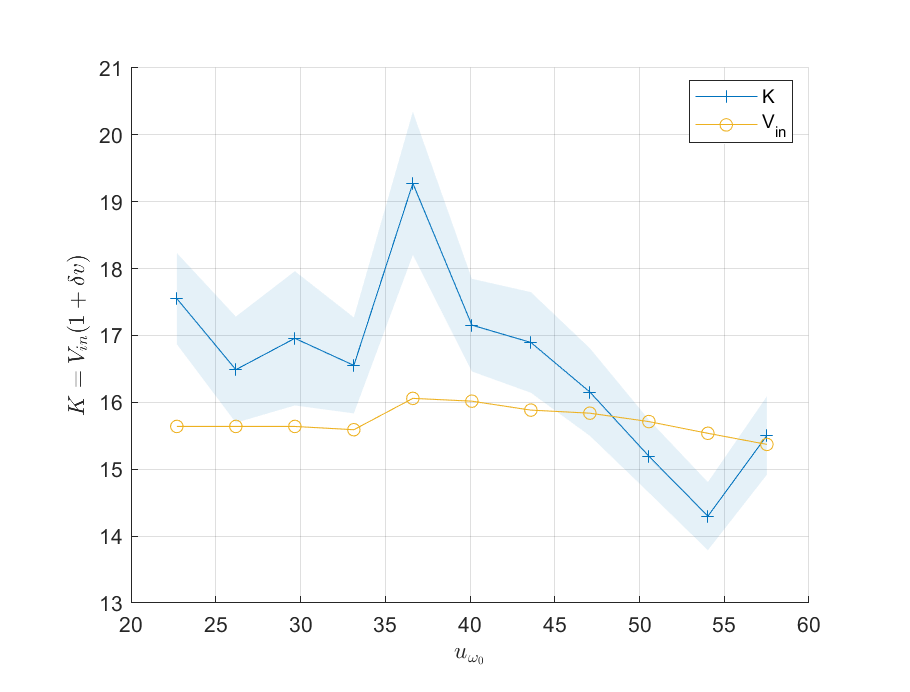
\includegraphics[width = \textwidth]{./figs/small_perturbation/K-Vin.eps}
            \caption{Static gain and Voltage input}
        \end{figure}
    \end{minipage}
    \begin{minipage}{0.49\textwidth}
        \begin{figure}[H]
            \includegraphics[width = \textwidth]{./figs/small_perturbation/omega_fit.eps}
            \caption{Cut-off frequency}
        \end{figure}
    \end{minipage}
\end{figure}



\subsubsection{Validation using the response of the full non-linear model}
We have the model parameters identified:
\begin{table}[H]
    \centering
    \begin{tabular}{c l l}
        \hline \hline
        Parameter & Value & \\ \hline \hline
        $C_T$ & $7.2581 \times 10^{-06}$ & $N/(rad/s)^2$  \\
        $C_D$ & $3.6088 \times 10^{-08}$ & $N.m/(rad/s)^2$ \\
        $b_m$ & $0.0$                    & $N.m/(rad/s)$\\
        $M_f$ & $1.3135 \times 10^{-3}$  & $N.m$\\
        $J$   & $3.2238 \times 10^{-6}$  & $Kg .m^2$ \\\hline \hline
    \end{tabular}
    \caption{Summary of parameter estimates from staic and small-perturbation experiments}
\end{table}

Assuming $\delta v = 0$ we have the non-linear model of the system eqn~\ref{eqn::nl_model}:
\begin{align*}
    J \dot \omega + b_m \omega + C_D \omega^2 = V_{in} b_m u_\omega + V_{in}^2 C_D u_\omega^2
\end{align*}
The above model is simulated with the identified parameters using a square wave and chirp input whose amplitude covers the full operating range. The results of the simulation are then compared with the experimental data.
\begin{figure}[H]
    \begin{minipage}{0.49\textwidth}
        \begin{figure}[H]
            \includegraphics[width = \textwidth]{./figs/nl_valid/square_validation.eps}
            \caption*{Square Wave Input}
        \end{figure}
    \end{minipage}
    \begin{minipage}{0.49\textwidth}
        \begin{figure}[H]
            \includegraphics[width = \textwidth]{./figs/nl_valid/chirp_validation.eps}
            \caption*{Chirp Input}
        \end{figure}
    \end{minipage}
    \caption{Model Validation}
    \label{fig::model_valid}
\end{figure}

Form the Figure~\ref{fig::model_valid}, it can be concluded that the model parameters are estimated with a reasonable accuracy. The error in simulation as compared to the esperiment can be primarily attributed to theh $\delta v$ that needs to me estimated in real-time.


%===============================================================================
\newpage
\part{Control}
\section{Control Model and Input}
From parameter estimates (Table~\ref{tab::parm_ests}), it can be seen that the
estimate of total 'damping' factor $( b_m )$ is zero. Thus, the linear term of
the control input in the RHS of eqn.~\ref{eqn::nl_model} can be ignored.
Let $u = u_\omega ^2 $ be the control input to the system for which we are going
to design the feedback controller. Incorporating the above two assumptions into
eqn.~\ref{eqn::nl_model}, we have the control form of the model:
\begin{equation} \label{eqn::control_form}
    J \dot \omega + b_m \omega + C_D \omega^2 + M_f \delta v = V_{in}^2 (1 + \delta v) C_D u
\end{equation}

We have the following bounds on the control input:
\begin{align*}
    u &= u_\omega^2 = \lr{a u_p + b}^2\\
    \implies u_{min} &= \lr{a u_{p_{min}}  + b}^2 = \lr{0.0696 \times 1110 - 64.3266}^2 = 167.1694\\
    \implies u_{max} &= \lr{a u_{p_{max}}  + b}^2 = \lr{0.0696 \times 1890 - 64.3266}^2 = 4518.1789\\
\end{align*}

The goal of feedback control design for the actuator is two-fold:
\begin{enumerate}
\item Compensate for the input-uncertainities, un-modelled disturbances and
model-structure errors.
\item Make the actuator track the response of a second-order transfer function
with no over-shoot of the form:
\begin{align*}
    G_{ref}(s) &= \frac{1}{s^2 + 2 \zeta \omega_{ref} + \omega_{ref}^2}
    && \zeta = \frac{1}{\sqrt{2}} = 0.707
\end{align*}
Such that, $\omega_{ref}$ results in the maximum possible bandwidth in presence
of uncertainties mentioned above.
\end{enumerate}

To this end, two feedback control designs based on Adaptive Robust Control
Theory (ARC) are implemented, and their performances are compared:
\begin{enumerate}
    \item Direct/Indirect Adaptive Robust Controller (DIARC).
    \item ARC design with parameter estimation only for the disturbances(Disturbance ARC).
    \item Feedback linearization.
\end{enumerate}

%===============================================================================
\subsection{Parametric model and parameter bounds for ARC design}

The parameter bounds are obtained from the variance of estimates and the
maximum value of $\delta v$. For the current design $\pm 2\sigma$ bounds are
used for each of the $\theta$'s. From experimental observations, the maximum
supply voltage is about $16\, V$ and minimum supply voltage is close to $15\,
V$. The average would be in the middle ($15.5\, V$). The physics dictates that
all the physical parameters have a non-negative value. Also, the minimum value
of $J$ is assumed to be $1/10$ of its nominal value instead of zero. This is to
ensure that the inertia estimate would never be zero and with-in the reasonable
limits. The following table gives the minimum, maximum and nominal values of the parameters:

\begin{table}[H]
    \centering
    \begin{tabular}{r l r r r}
        \hline \hline
        Parameter & Units &Nominal & Minimum & Maximum \\ \hline \hline
        $C_T$                   &
        $N/(rad/s)^2$           &
        $7.2581e-6$             &
        $7.1690e-6$             &
        $7.3471e-6$
        \\
        $C_D$                   &
        $N.m/(rad/s)^2$         &
        $3.6088e-8$             &
        $3.3295e-8$             &
        $3.8881e-8$

        \\
        $b_m$                    &
        $N.m/(rad/s)$            &
        $0$                      &
        $0$                      &
        $9.2006e-6$
        \\
        $M_f$                    &
        $N.m$                    &
        $1.3135e{-3}$            &
        $0$                      &
        $0.0104$
        \\
        $J$                      &
        $Kg.m^2$                 &
        $3.2238e{-6}$            &
        $3.2238e{-7}$            &
        $1.7234e-5$
        \\
        $V_{in}$                 &
        $V$                      &
        $15.5$                   &
        $15$                     &
        $16$
        \\
        $\delta v$               &
                                 &
        $0$                      &
        $-0.2$                   &
        $0.2$
        \\
        \hline \hline
    \end{tabular}
    \caption{Summary of parameter bounds}
    \label{tab::parm_bounds}
\end{table}

\subsubsection{Parametric Model}
It can be noted that the variance of $\hat J$ is substantial as compared to its
actual value. This would propagate into the all the parameters if it is divided
on all sides. Instead, we normalize all the coefficients with the controller
gain to minimize the propagation of variance to the parameters. Thus,
eqn.~\ref{eqn::control_form} becomes:

\begin{align*}
    \lr{\frac{J}{V_{in}^2 C_D}} \dot \omega + \lr{\frac{b_m}{V_{in}^2 C_D}} \omega + \lr{\frac{1}{V_{in}^2}} \omega^2  &= u + \delta v \lr{u - \frac{M_f}{V_{in}^2 C_D}}\\
    %===
    \text{Let, } \qquad &\\
    \theta_1 = \lr{\frac{J}{V_{in}^2 C_D}} \qquad
    \theta_2 &= \lr{\frac{b_m}{V_{in}^2 C_D}}\qquad
    \theta_3 = \lr{\frac{1}{V_{in}^2}}\\
    d(t) &= \delta v \lr{u - \frac{M_f}{V_{in}^2 C_D}}\\
    %===
    \implies \theta_1 \dot \omega + \theta_2 \omega + \theta_3 \omega^2 &= u + d(t)
\end{align*}
\begin{equation}\label{eqn::almst_ctrl_mdl}
    \theta_1 \dot \omega = u - \theta_2 \omega - \theta_3 \omega^2 + d(t)
\end{equation}

Let, $\omega_d(t)$ be the desired trajectory that the system needs to track
(output of $G_{ref}(s)$). Thus, the tracking error:
\begin{align*}
    s &= \omega - \omega_d \quad \implies \dot s = \dot \omega - \dot \omega_d
\end{align*}
Dividing the disturbance into high-frequency component and a slowly varying
component, let, $$d(t) = d_0 + \Delta(t)$$
Thus, subtracting $\theta_1 \omega_d$ on both sides of eqn.~\ref{eqn::almst_ctrl_mdl}.
\begin{align*}
    \theta_1 (\dot \omega - \dot \omega_d) &= u - \theta_1 \omega_d - \theta_2 \omega - \theta_3 \omega^2 + d_0 + \Delta(t)\\
    \text{Let,} \qquad\\
    \pmb \theta &= \bm{\theta_1 & \theta_2 & \theta_3 & d_0}^T\\
    \pmb \phi &= \bm{-\omega_d & -\omega & - \omega^2 & 1}^T\\
\end{align*}
Thus we have the model for tracking error dynamics:
\begin{equation}\label{eqn::error_dyn}
    \theta_1 \dot s = u + \pmb \phi^T \pmb \theta + \Delta(t)
\end{equation}


\subsubsection{Parameter Bounds}
The parameter bounds for eqn.~\ref{eqn::error_dyn} are obtained from the
parameter bounds of estimated parameters. Also,
\begin{align*}
    \abs{d(t)} &\leq d_M \implies \abs{d_0} \leq d_M \text{  and  } \abs{\Delta} \leq 2d_M = \Delta_M\\
    \text{From Table~\ref{tab::parm_bounds}} \qquad &\\
    d_M &= \delta v_{max} \lr{u_{max} - \frac{M_{f_{min}}}{V_{in_{max}}^2 C_{D_{max}}}} \approx 900
\end{align*}
Similarly, we have
\begin{table}[H]
    \centering
    \begin{tabular}{r l r r r}
        \hline \hline
        Parameter & Equation & Nominal & Minimum & Maximum\\ \hline \hline
        $\theta_1$ &
        $= \lr{\frac{J}{V_{in}^2 C_D}}$ &
        $3.7183e-1$ &
        $3.2388e-2$ &
        $2.3005$
        \\
        $\theta_2$ &
        $= \lr{\frac{b_m}{V_{in}^2 C_D}}$ &
        $0$ &
        $0$ &
        $1.0794$
        \\
        $\theta_3$ &
        $= \lr{\frac{1}{V_{in}^2}}$ &
        $4.1623e-3$ &
        $3.9062e-3$ &
        $4.4444e-3$
        \\
        \hline \hline
    \end{tabular}
    \caption{Parameter Bounds}
    \label{tab::parm_lims}
\end{table}

%===============================================================================
\newpage
\section{Direct Adaptive Robust Control Design (DARC)}
\subsection{Direct-Indirect Adaptive Robust Control Design (DIARC)}
\subsection{Adaptive Robust Control Design (ARC) with only disturbance estimation}

%===============================================================================
% \newpage
% \section{Disturbance Observer based Controller Designs}
% \subsection{DOB Design}
% \subsection{Active Disturbance Rejection Controller Design (ADRC)}

% %===============================================================================
% \newpage
% \section{Comparative Study}

%===============================================================================
\newpage
\section{Conclusion}
\newpage
\section{Appendix}
\subsection{Linearized Model Validation \label{sec::small_perturb_valid}}

\subsubsection{Frequency Domain Validation}
%===============================================================================
\begin{figure}[H]
    \begin{minipage}{0.32\textwidth}
       \begin{figure}[H]
            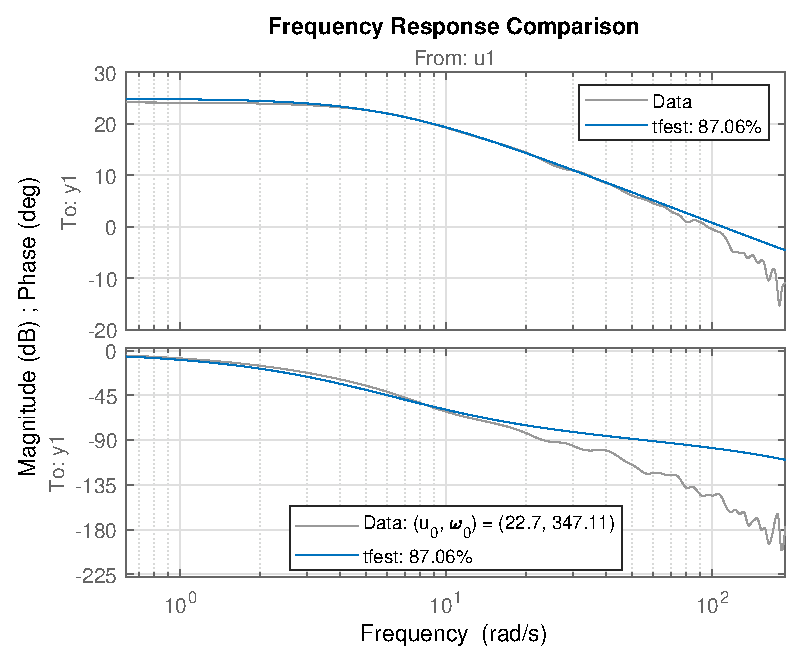
\includegraphics[width = \textwidth]{./figs/small_perturbation/freq_Compare_1250.eps}
       \end{figure}
    \end{minipage}
    \begin{minipage}{0.32\textwidth}
       \begin{figure}[H]
            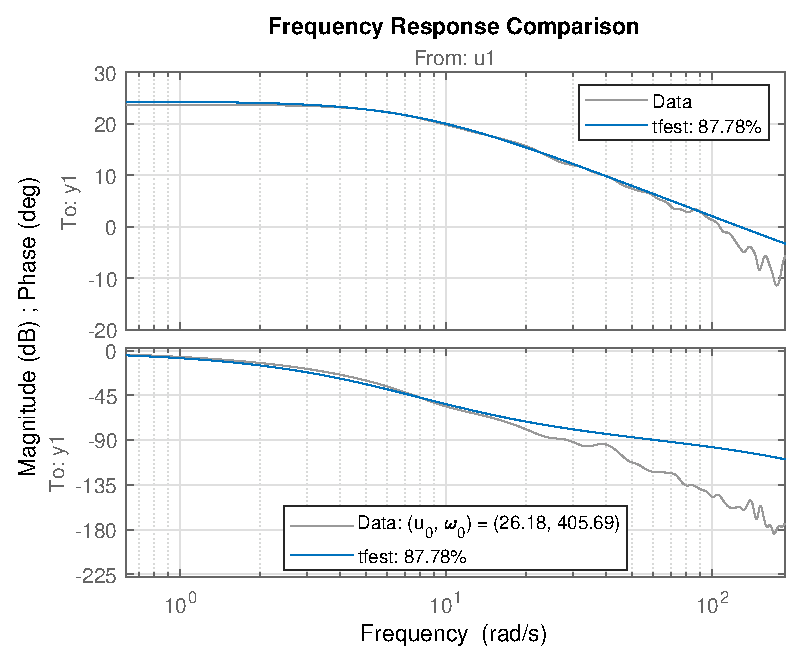
\includegraphics[width = \textwidth]{./figs/small_perturbation/freq_Compare_1300.eps}
       \end{figure}
    \end{minipage}
    \begin{minipage}{0.32\textwidth}
       \begin{figure}[H]
            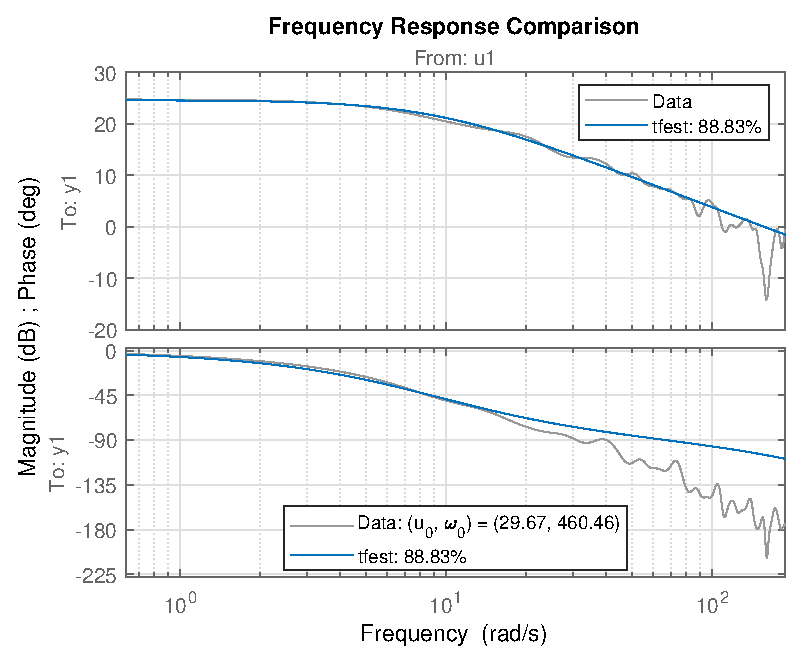
\includegraphics[width = \textwidth]{./figs/small_perturbation/freq_Compare_1350.eps}
       \end{figure}
    \end{minipage}
\end{figure}
%-------------------------------------------------------------------------------
\begin{figure}[H]
    \begin{minipage}{0.32\textwidth}
       \begin{figure}[H]
            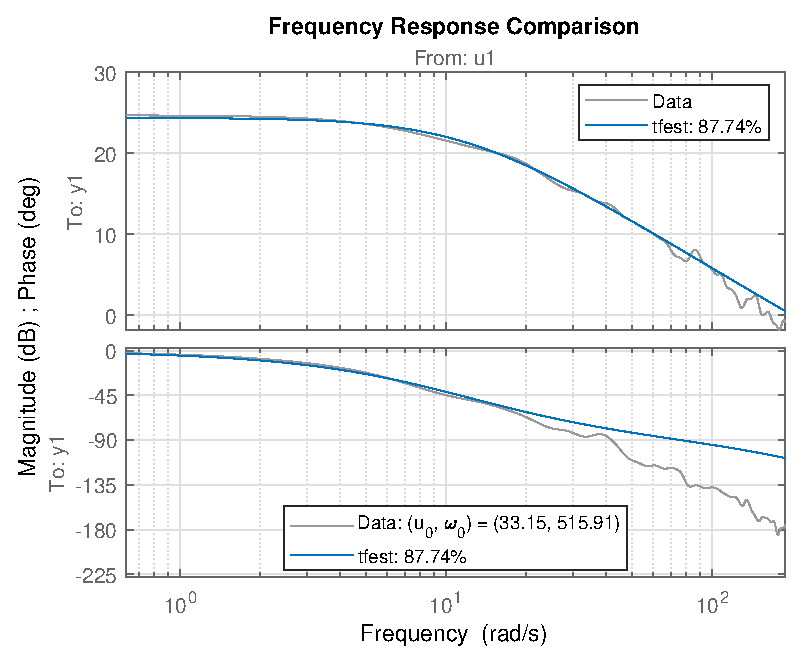
\includegraphics[width = \textwidth]{./figs/small_perturbation/freq_Compare_1400.eps}
       \end{figure}
    \end{minipage}
    \begin{minipage}{0.32\textwidth}
       \begin{figure}[H]
            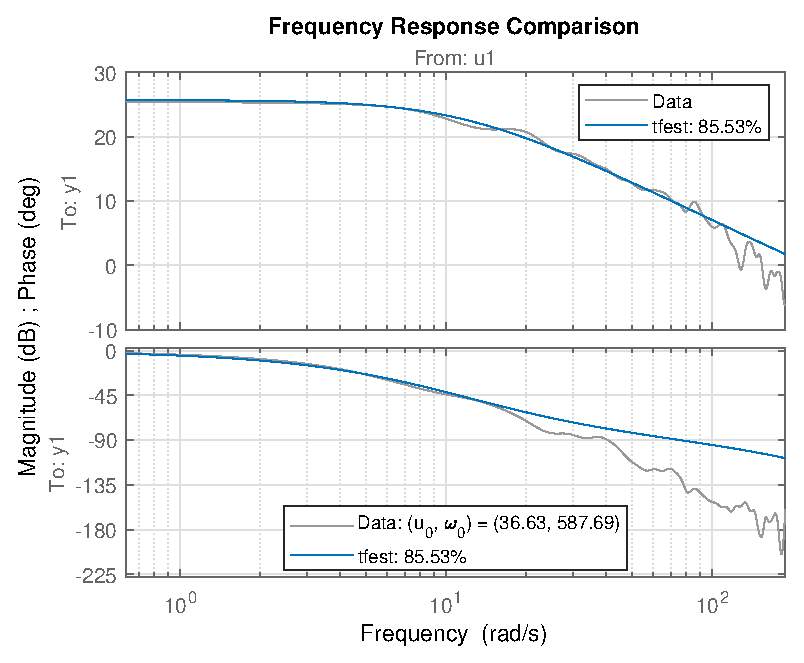
\includegraphics[width = \textwidth]{./figs/small_perturbation/freq_Compare_1450.eps}
       \end{figure}
    \end{minipage}
    \begin{minipage}{0.32\textwidth}
       \begin{figure}[H]
            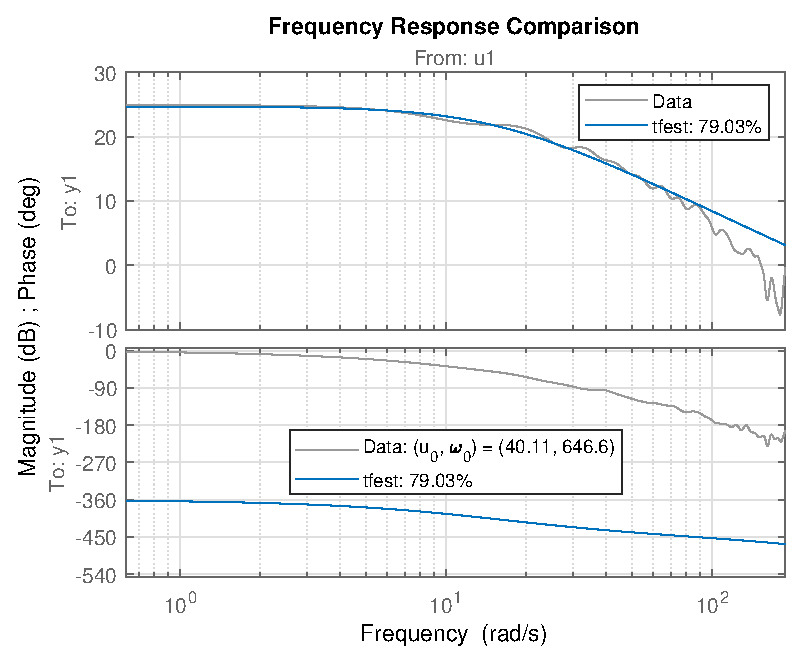
\includegraphics[width = \textwidth]{./figs/small_perturbation/freq_Compare_1500.eps}
       \end{figure}
    \end{minipage}
\end{figure}
%-------------------------------------------------------------------------------
\begin{figure}[H]
    \begin{minipage}{0.32\textwidth}
       \begin{figure}[H]
            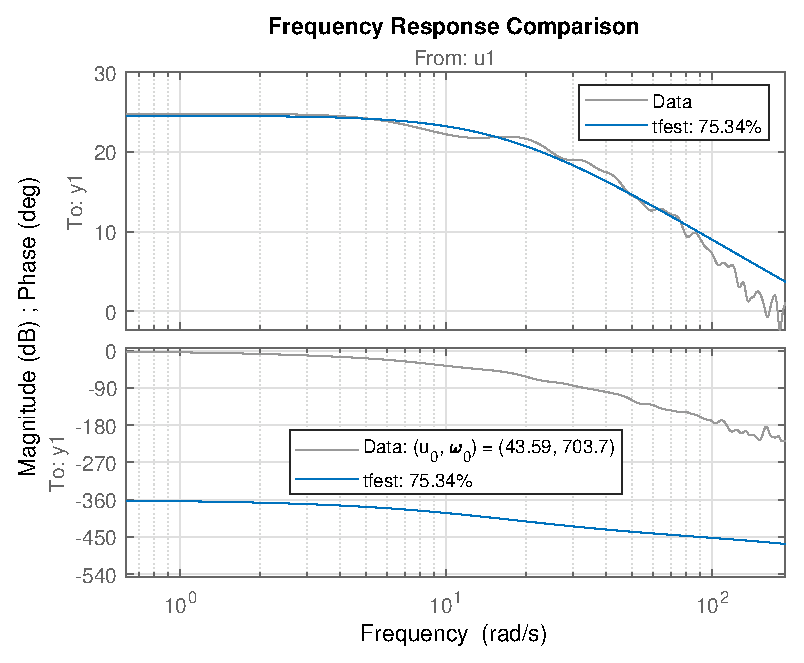
\includegraphics[width = \textwidth]{./figs/small_perturbation/freq_Compare_1550.eps}
       \end{figure}
    \end{minipage}
    \begin{minipage}{0.32\textwidth}
       \begin{figure}[H]
            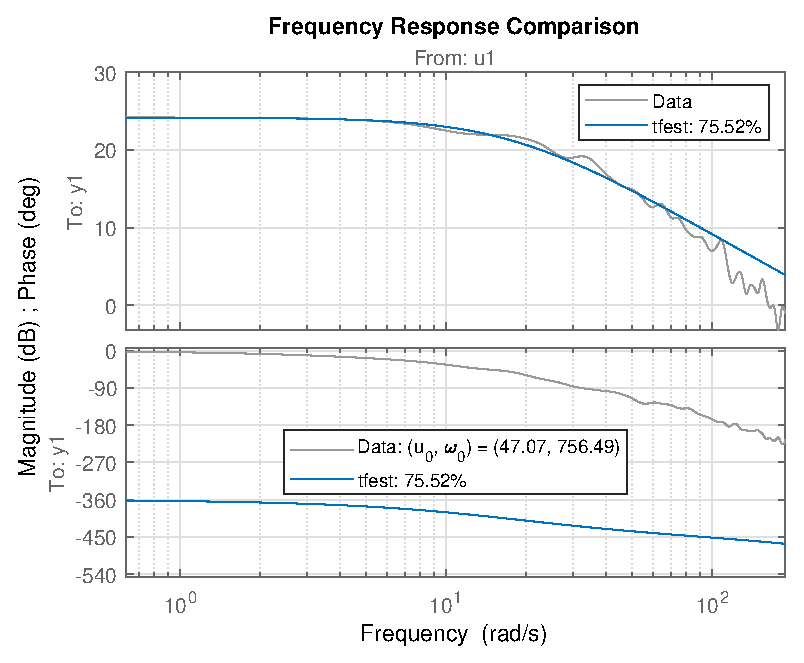
\includegraphics[width = \textwidth]{./figs/small_perturbation/freq_Compare_1600.eps}
       \end{figure}
    \end{minipage}
    \begin{minipage}{0.32\textwidth}
       \begin{figure}[H]
            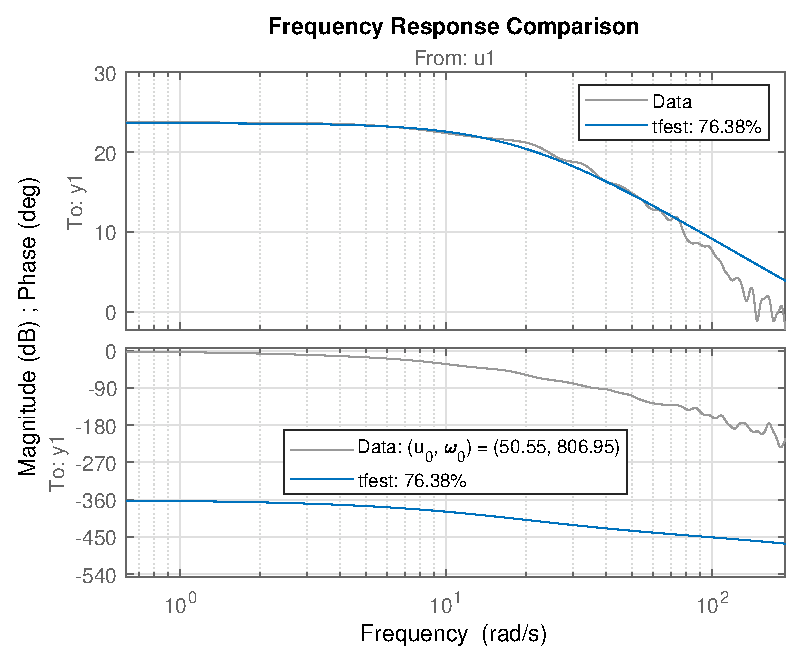
\includegraphics[width = \textwidth]{./figs/small_perturbation/freq_Compare_1650.eps}
       \end{figure}
    \end{minipage}
\end{figure}
%-------------------------------------------------------------------------------
\begin{figure}[H]
    \centering
    \begin{minipage}{0.32\textwidth}
       \begin{figure}[H]
            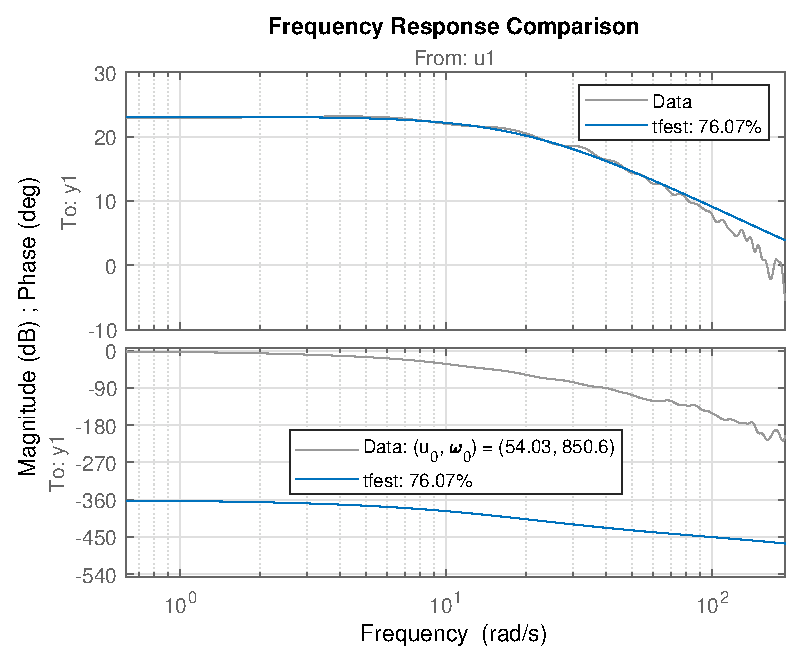
\includegraphics[width = \textwidth]{./figs/small_perturbation/freq_Compare_1700.eps}
       \end{figure}
    \end{minipage}
    \begin{minipage}{0.32\textwidth}
       \begin{figure}[H]
            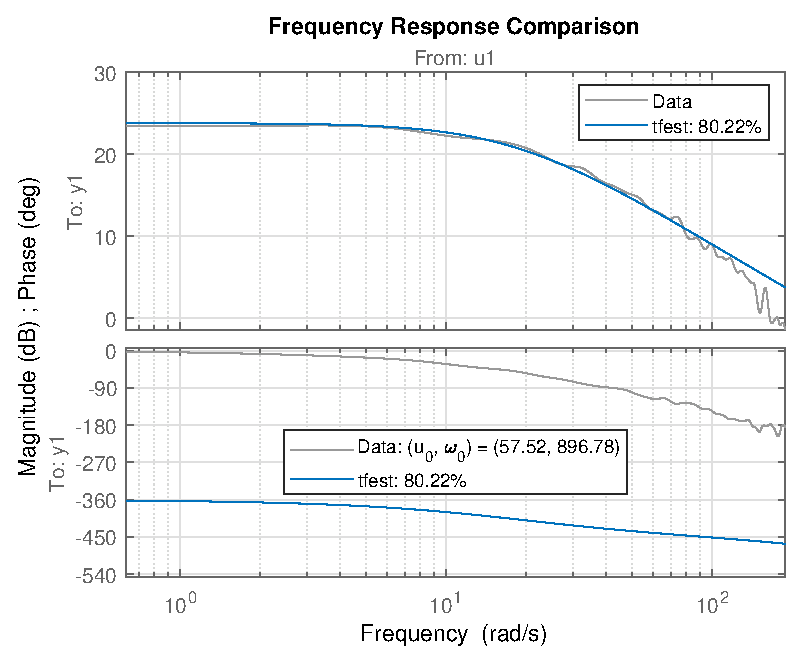
\includegraphics[width = \textwidth]{./figs/small_perturbation/freq_Compare_1750.eps}
       \end{figure}
    \end{minipage}
\end{figure}


\subsubsection{Time Domain Validation}
%===============================================================================
\begin{figure}[H]
    \begin{minipage}{0.32\textwidth}
       \begin{figure}[H]
            \includegraphics[width = \textwidth]{./figs/small_perturbation/time_Compare_1250.eps}
       \end{figure}
    \end{minipage}
    \begin{minipage}{0.32\textwidth}
       \begin{figure}[H]
            \includegraphics[width = \textwidth]{./figs/small_perturbation/time_Compare_1300.eps}
       \end{figure}
    \end{minipage}
    \begin{minipage}{0.32\textwidth}
       \begin{figure}[H]
            \includegraphics[width = \textwidth]{./figs/small_perturbation/time_Compare_1350.eps}
       \end{figure}
    \end{minipage}
\end{figure}
%-------------------------------------------------------------------------------
\begin{figure}[H]
    \begin{minipage}{0.32\textwidth}
       \begin{figure}[H]
            \includegraphics[width = \textwidth]{./figs/small_perturbation/time_Compare_1400.eps}
       \end{figure}
    \end{minipage}
    \begin{minipage}{0.32\textwidth}
       \begin{figure}[H]
            \includegraphics[width = \textwidth]{./figs/small_perturbation/time_Compare_1450.eps}
       \end{figure}
    \end{minipage}
    \begin{minipage}{0.32\textwidth}
       \begin{figure}[H]
            \includegraphics[width = \textwidth]{./figs/small_perturbation/time_Compare_1500.eps}
       \end{figure}
    \end{minipage}
\end{figure}
%-------------------------------------------------------------------------------
\begin{figure}[H]
    \begin{minipage}{0.32\textwidth}
       \begin{figure}[H]
            \includegraphics[width = \textwidth]{./figs/small_perturbation/time_Compare_1550.eps}
       \end{figure}
    \end{minipage}
    \begin{minipage}{0.32\textwidth}
       \begin{figure}[H]
            \includegraphics[width = \textwidth]{./figs/small_perturbation/time_Compare_1600.eps}
       \end{figure}
    \end{minipage}
    \begin{minipage}{0.32\textwidth}
       \begin{figure}[H]
            \includegraphics[width = \textwidth]{./figs/small_perturbation/time_Compare_1650.eps}
       \end{figure}
    \end{minipage}
\end{figure}
%-------------------------------------------------------------------------------
\begin{figure}[H]
    \centering
    \begin{minipage}{0.32\textwidth}
       \begin{figure}[H]
            \includegraphics[width = \textwidth]{./figs/small_perturbation/time_Compare_1700.eps}
       \end{figure}
    \end{minipage}
    \begin{minipage}{0.32\textwidth}
       \begin{figure}[H]
            \includegraphics[width = \textwidth]{./figs/small_perturbation/time_Compare_1750.eps}
       \end{figure}
    \end{minipage}
\end{figure}


%===============================================================================
%\newpage
%===============================================================================
\newpage
\bibliographystyle{unsrt}
\bibliography{refs}

\end{document}
